                                                                                                        %\pdfoutput=1
%\documentclass[fms,times]{cuparticle}
\documentclass[a4paper,11pt,twoside]{amsart}
\usepackage{amsmath}
\usepackage{geometry}
%\newproof{proof}{Proof}
\usepackage{amssymb, latexsym}
\usepackage{appendix}
\usepackage{verbatim}
%\usepackage{amscd}
\usepackage{enumerate}
\usepackage{comment}
\usepackage{txfonts}
\usepackage{float}
\usepackage{parskip}
\usepackage{lipsum}
	
%\usepackage[breaklinks=true,hidelinks]{hyperref}

%\usepackage{psfig}
%\usepackage{graphicx}
%\usepackage{showkeys}  
%\usepackage{siunitx}
%\usepackage{tikz-cd}
%\usepackage{color}
%\usetikzlibrary{arrows}
% uncomment this when editing cross-references
%\numberwithin{equation}{section}
%\usepackage{hyperref}

%\volume{}
%\doi{}


% \usepackage{mathabx}


\usepackage{mathtools}%                  http://www.ctan.org/pkg/mathtools
\usepackage[tableposition=top]{caption}% http://www.ctan.org/pkg/caption
\usepackage{booktabs,dcolumn}%           http://www.ctan.org/pkg/dcolumn + http://www.ctan.org/pkg/booktabs
\usepackage[symbol]{footmisc}

\geometry{a4paper,total={6in,8in}, margin=1in}
\interfootnotelinepenalty=10000
     
%\theoremstyle{plain}

\newtheorem{theorem}{Theorem}[section]
%\newtheorem{theorem}[theorem]{Theorem}
\newtheorem{proposition}[theorem]{Proposition}
\newtheorem{hypothesis}[theorem]{Hypothesis}
\newtheorem{lemma}[theorem]{Lemma}
\newtheorem{corollary}[theorem]{Corollary}
\newtheorem{conjecture}[theorem]{Conjecture}
\newtheorem{principle}[theorem]{Principle}
\newtheorem{claim}[theorem]{Claim}

%\theoremstyle{definition}

%\newtheorem{roughdef}[subsection]{Rough Definition}
\newtheorem{definition}[theorem]{Definition}
\newtheorem{remark}[theorem]{Remark}
\newtheorem{remarks}[theorem]{Remarks}
\newtheorem{example}[theorem]{Example}
\newtheorem{examples}[theorem]{Examples}
%\newtheorem{problem}[subsection]{Problem}
%\newtheorem{question}[subsection]{Question}

\newcommand\F{\mathbb{F}}
\newcommand\E{\mathbb{E}}
\newcommand\R{\mathbb{R}}
\newcommand\Z{\mathbb{Z}}
\newcommand\N{\mathbb{N}}
\newcommand\D{\mathbb{D}}
\newcommand\C{\mathbb{C}}
\newcommand\Q{\mathbb{Q}}
\newcommand\T{\mathbb{T}}

\newcommand\e{\mathrm{e}}
\newcommand\Ei{\mathrm{Ei}}
\newcommand\IL{\mathrm{IL}}
\newcommand\li{\mathrm{li}}
\newcommand\Li{\mathrm{Li}}
\newcommand\PV{\mathrm{PV}}
\newcommand\Res{\mathrm{Res}}
\newcommand\RL{\mathrm{RL}}

\renewcommand\Re{{\operatorname{Re\,}}}
\renewcommand\Im{{\operatorname{Im\,}}}
\renewcommand{\thefootnote}{\fnsymbol{footnote}}
\newcommand\Log{{\operatorname{Log}}}
\newcommand\eps{\varepsilon}



\renewcommand\P{\mathbf{P}}


%%%%%%%%%%%%%%%%%%%%%%%%%%%%%%%%


\newcommand{\alert}[1]{{\bf \color{red} TODO: #1}}


\setlength\evensidemargin\oddsidemargin
%\setlength{\parindent}{0cm}

\usepackage{color}
\definecolor{almond}{rgb}{0.94,0.87,0.8}

\let\oldv\verbatim
\let\oldendv\endverbatim

\def\verbatim{\par\setbox0\vbox\bgroup\oldv}
\def\endverbatim{\oldendv\egroup\fboxsep0pt \noindent\colorbox[gray]{0.8}{\usebox0}\par}

\begin{document}
\title[Extending the logarithmic integral]{EXTENDING THE LOGARITHMIC INTEGRAL: AN EXPLORATION OF INTEGRALS OF POWERS OF THE RECIPROCAL OF THE LOG-FUNCTION}

\author{Kalpesh Muchhal, Rudolph Dwars \\ \\ \textit{March 18, 2023,  \,\, Version 1.1}}
\address{\tt{{\it E-mail Address}: ra.dwars@quicknet.nl}}
\address{\tt{{\it E-mail Address}: kalpesh.muchhal@iitbombay.org}}


\begin{abstract}
In this paper we investigate functions of the kind:
$L(y,x) = \int_0^x \frac{1}{\log^y t} dt$.
The case for $y=1$ is the well known function $\li(x)$ which also features in Riemann's explicit formula for the prime counting function. For $y>1$, $L(y,x)$ shows interesting properties which we explore both numerically and analytically.
\end{abstract}

\maketitle

\section{Introduction}

Our starting point for this paper is the expression below derived through integration by parts of the well known logarithmic integral \cite{edwr}, defined for $x>1$ in the Cauchy Principal Value (CPV) sense

\begin{equation}\label{li1}
 \PV \int_0^x \frac{1}{\log t} dt = \frac{x}{\log x} + \PV
\footnote[1]{\textit{It is a somewhat interesting question in its own right whether the $\PV$ notation should be used where non-simple poles are involved. The conventional definition of Cauchy Principal Value for a function f(x) with a pole at c is $\int\limits_a^{c-\epsilon} f(x) dx + \int\limits_{c+\epsilon}^{b} f(x) dx$, with $\epsilon \to 0$, and under this definition, the CPV diverges for a non-simple pole. However, as seen in the next section, the alternate method of contour integrals for calculating the CPV for a simple pole easily extends to non-simple poles, and it is in this sense that we retain the $\PV$ notation.}}
\int_0^x \frac{1}{\log^2 t} dt
\end{equation}

Using $L(y,x) = \PV \int_0^x \frac{1}{\log^y t} dt$, this can be compactly written as 
$L(1,x) = \frac{x}{\log x} + L(2,x)$,
from which we see that $L(2,x)$ is finite due to its relation with $L(1,x)$.

By repeated integration by parts, we also see that $L(1,x)$ has an asymptotic expansion in terms of $L(y,x)$ terms, and that in general $L(y,x)$ is finite, since it can be expressed recursively in terms of $L(y-1,x)$ for $y$ an integer greater than $1$.
\begin{align}
L(1,x) &= x\sum\limits_{k=1}^{y-1} \frac{(k-1)!}{\log^{k} x} + ((y-1)!)\,L(y,x)  \\
L(y,x) &= \frac{1}{y-1} \, \left(L(y-1,x) - \frac{x}{\log^{y-1} x}\right) \\
\notag
\end{align}
Since $L(1,2) = \li(2) \approx 1.04516...$ \cite{weis} is known historically (one reason being its importance in prime counting formulas), the recursion formula can then be used to compute any $L(y,x)$ for $y$ integer. For eg. keeping $x=2$ and varying $y$, we get
\begin{table}[H]
  \begin{tabular}{r|r} % <-- Alignments: 1st column left, 2nd middle and 3rd right, with vertical lines in between
      $y$ & L(y,2)\\
      \hline
      2 & -1.84023\\
      3 & -3.00148\\
      4 & -3.00235\\
      5 & -2.91664\\
      6 & -3.08328\\
  \end{tabular}
  \caption{Sample values of $L(y,2)$}
\end{table}
\vspace{-2em}

Some remarks on notation and convention used later in the paper:
\begin{itemize}
 \item exponent n $->$ emphasizes integer exponents
 \item exponent q $->$ emphasizes real exponents including integers
 \item AUC $->$ Area Under the Curve obtained through real integration
 \item PV, CPV $->$ Cauchy Principal Value obtained through complex integration 
 \item $\mu_y$ $->$ Solution of $L(y,x)=0$
\end{itemize}

\section{Evaluation of $L(n,2)$ using contour integration}

In the earlier section, we computed $L(n,x)$ using $\li(x)$, but we can also compute it directly using contour integration. In fact, given an $n$ and $x$, we compute $L(n,x)$ using several different contours to always arrive at the same estimate, showing CPV when computed this way is a well defined concept even when higher order poles are involved. 

As shown in the figure below, for CPV calculations, we use a closed semicircular contour ABCDEFA that excludes the singularity at $z=1$
\begin{itemize}
 \item ABC is an upper semicircle of radius r (with r being finite) centred at $z=1$,
 \item DEF is an upper semicircle of radius $\epsilon$ (where $\epsilon -> 0$).
 \item and two straight line segments AF and DC each of length x-$\epsilon$.
\end{itemize}
There are also two additional straight line segments A'A and CC' outside the closed contour, each of length $1-r$.

\begin{figure}[H]
  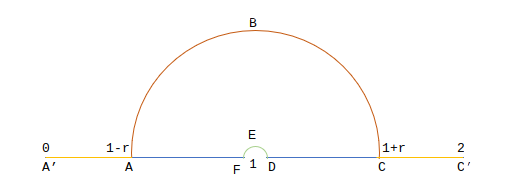
\includegraphics[width=0.5\linewidth]{contour_diagram_label2.png}
  \caption{Contour construction to evaluate $L(n,2)$}
\end{figure}

Since the segments A'A and CC' do not contain a singularity, their AUC (area under the curve) and CPV estimates are always equal. But these estimates differ in general for the segment AC, which has a singularity at $z=1$. $$\PV \int\limits_{A'}^{C'} f(x)\, dx = \int\limits_{A'}^{A} f(x)\, dx + \PV \int\limits_{A}^{C} f(x) \,dx + \int\limits_{C}^{C'}f(x)\, dx$$

Since the contour ABCDEFA does not contain a singularity, and the open arc DEF contributes to the residue term in proportion to its arc length, we have: $$\PV \int\limits_{A}^{C} f(x)\, dx = \int\limits_{ABC} f(x)\, dx + \int\limits_{DEF} f(x)\, dx$$ Hence,
$$\PV \int\limits_{0}^{2} f(x)\, dx = \left(\int\limits_{0}^{1-r} f(x)\, dx + \int_{1+r}^{2} f(x) \,dx \right) - \left(\int\limits_{0}^{\pi} i \exp(i \theta)f(1+\exp(i\theta)) \, d{\theta}\right) + \pi i\, \Res(f(z),1)$$

Firstly let $y=1$, the case of the simple pole.

\begin{table}[H]
  \begin{center}
    \begin{tabular}{r|r|r|r|r} % <-- Alignments: 1st column left, 2nd middle and 3rd right, with vertical lines in between
      $r$ & AUC A'A & AUC CC' & CPV AC & CPV A'C'\\
      \hline
      1 & 0 & 0 & 1.045164 & 1.045164\\
      0.5 & -0.37867 & 0.92010 & 0.50374 & 1.045164\\
      0.3 & -0.78095 & 1.52534 & 0.30077 & 1.045164\\
      0.1 & -1.77580 & 11.37681 & 0.10003 & 1.045164\\
      0.001 & -6.33104 & 1005.99020 & 0.00100 & 1.045164\\
      0.00001 & -10.93571 & 11.98087 & 0.00001 & 1.045164\\
    \end{tabular}
  \end{center}
  \caption{AUC and CPV breakup of $L(1,2)$}
\end{table}
\vspace{-2em}
We can observe in the simple pole case that as the radius $r$ decreases, the CPV also decreases towards 0. AUC of the A'A and CC' segments decrease/increase without bound, but symmetrically. It is due to these two properties, that the $\epsilon$-method for CPV works with simple poles, but as seen below does not work for non-simple poles.   

Let $y=2$. The singularity at $x=1$ is now a higher order pole with order 2. $\frac{1}{\log^{2}x}$ is always positive on the real line and when we plot it, we see that the the area under the curve AUC is infinite. However, as seen earlier, CPV is finite, and we reconcile these twin phenomena below. 

\begin{figure}[H]
  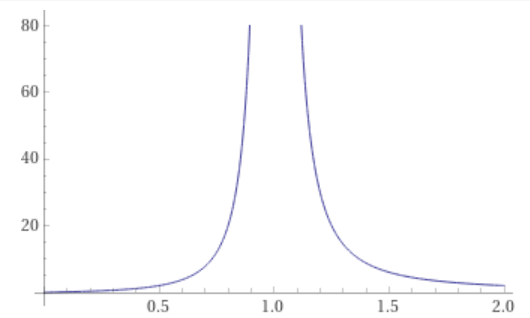
\includegraphics[width=0.5\linewidth]{l22_auc.png}
  \caption{AUC of L(2,2)}
\end{figure}

The residue for an $n$th order pole for a function $g(z)$ can be calculated analytically as: 
$$\frac{1}{(n-1)!} \lim_{z->c} \frac{d^{n-1}}{dz^{n-1}} ((z-c)^{n} g(z))$$ or more intuitively from the Laurent expansion of $g(z)$, as shown in a later section.

The other three terms in the $\PV$ formula are calculated numerically.

\begin{table}[H]
  \begin{center}
    \begin{tabular}{r|r|r|r|r} % <-- Alignments: 1st column left, 2nd middle and 3rd right, with vertical lines in between
      $r$ & AUC A'A & AUC CC' & CPV AC & CPV A'C'\\
      \hline
      1 & 0 & 0 & -1.84023 & -1.84023\\
      0.5 & 0.34268 & 1.73416 & -3.91707 & -1.84023\\
      0.3 & 1.18162 & 3.59489 & -6.61674 & -1.84023\\
      0.1 & 6.76630 & 11.37681 & -19.98334 & -1.84023\\
      0.001 & 992.16938 & 1005.99020 & -19999.99983 & -1.84023\\
      0.00001 & 99987.564 & 100010.595 & -199999.99999 & -1.84023\\
    \end{tabular}
    \caption{AUC and CPV breakup of $L(2,2)$}
  \end{center}
\end{table}
\vspace{-2em}
As we decrease the radius $r$ of the semicircle ABC, we see as expected the AUC of the outer segments increasing without bound, but the CPV of the contour segment AC also increases negatively without bound, such that the total CPV of A'C' remains finite and constant.

Next, we evaluate the case of $L(3,2)$
\begin{table}[H]
  \begin{center}
    \begin{tabular}{r|r|r|r|r} % <-- Alignments: 1st column left, 2nd middle and 3rd right, with vertical lines in between
      $r$ & AUC A'A & AUC CC' & CPV AC & CPV A'C'\\
      \hline
      1 & 0 & 0 & -3.00148 & -3.00148\\
      0.5 & -0.34900 & 3.34770 & -6.00018 & -3.00148\\
      0.3 & -2.16039 & 9.15895 & -10.00004 & -3.00148\\
      0.1 & -37.15432 & 64.15285 & -30.00000 & -3.00148\\
      0.001 & -498504.4569 & 501501.4555 & -3000.0000 & -3.00148\\
      0.00001 & -4999850006.760 & 5000150003.758 & -300000.000 & -3.00148\\
    \end{tabular}
    \caption{AUC and CPV breakup of $L(3,2)$}
  \end{center}
\end{table}
\vspace{-2em}
Here we see on decreasing $r$, that the AUC of the left outer segment A'A approaches negative infinity, while that of the right outer segment CC' approaches positive infinity. But unlike in the L(1,2) case, they do not so symmetrically and hence their sum diverges. The CPV of the contour segment AC counterbalances this effect, such that CPV of the overall segment A'C' remains constant. 

\section{Laurent series expansion of $\frac{1}{\log^n z}$ for integer $n$}

Using the Laurent series expansion of $\frac{1}{\log z}$, we can use the multinomial theorem to get the corresponding expansion for $\frac{1}{\log^{n} z}$. This can then be used to easily get the residue for the latter expression at $z=1$.

Let $f(z)$ be a function with a simple pole, represented as a Laurent series as: $$f(z) = \frac{a_{-1}}{z-c} + a_0 + a_1 (z-c) + a_2 (z-c)^2 + ...$$
Then $$(f(z))^n = \frac{1}{(z-c)^n} \sum\limits_{k=0}^{\infty}(\sum\limits_{\substack{t_{-1} + t_0 + t_1 + ... t_{k-1} = n \\ 0t_{-1} + 1t_0 + 2t_1 + ... kt_{k-1} = k}} \frac{n!}{t_{-1}!t_{0}!t_{1}!...t_{k-1}!} a_{-1}^{t_{-1}} a_{0}^{t_0}a_{1}^{t_1}..a_{k-1}^{t_{k-1}} (z-c)^k)$$

Extracting the coefficient of $(z-c)^{-1}$, we get:
$$\Res((f(z))^n,c) =  
\sum\limits_{\substack{t_{-1} + t_0 + t_1 + ... t_{n-2} = n \\ 0t_{-1} + 1t_0 + 2t_1 + ... (n-1)t_{n-2} = n-1}} \frac{n!}{t_{-1}!t_{0}!t_{1}!...t_{n-2}!} a_{-1}^{t_{-1}} a_{0}^{t_0}a_{1}^{t_1}..a_{n-2}^{t_{n-2}}$$
 
Also since $\frac{1}{\log(z)} = \frac{1}{z-1} + \frac{1}{2} - \frac{1}{12} (z-1) + \frac{1}{24}(z-1)^2 - \frac{19}{720}(z-1)^3 + ...$ we can tabulate the residues at $z=1$ for the first few powers of $\frac{1}{\log(z)}$:

\begin{table}[H]
  \begin{center}
    \begin{tabular}{r|r|r} % <-- Alignments: 1st column left, 2nd middle and 3rd right, with vertical lines in between
      $n$ & $\Res((f(z))^n,c)$ &  $\Res(\frac{1}{\log^{n}(z)},1)$\\
      \hline
      1 &  $a_{-1}$ & 1\\
      2 &  $2a_{-1}a_{0}$ & 1\\
      3 &  $3a_{-1}^2 a_{1} + 3a_{-1} a_{0}^2$ & $\frac{1}{2!}$\\
      4 &  $4a_{-1}^3 a_{2} + 12a_{-1}^2 a_{0} a_{1} + 4a_{-1} a_{0}^3$ & $\frac{1}{3!}$\\
      5 &  $5a_{-1}^4 a_{3} + 20a_{-1}^3 a_{0} a_{2} + 10a_{-1}^3 a_{1}^2 + 30a_{-1}^2 a_{0}^2 a_{1} + 5a_{-1} a_{0}^4$ & $\frac{1}{4!}$\\
      .. & .. & ..\\
      n & .. & $\frac{1}{(n-1)!}$
    \end{tabular}
    \caption{Residues of a function's powers in terms of Laurent coefficients of the function}
  \end{center}
\end{table}
\vspace{-2em}
The symbolic formulas in the 2nd column above are valid for any function f(z)'s powers, with f(z) having a simple pole at c. Observing the 3rd column, $\Res(\frac{1}{\log^{n}(z)},1)$ has a nice property of evaluating to $\frac{1}{(y-1)!}$, but other functions (for e.g. the Riemann zeta function, which also has a simple pole at $z=1$) do not have such simply structured residues, as we will see in a later paper. 

\section{Roots of L(n,x) for integer n}

Since $\frac{1}{\log^{n} x}$ has a lone singularity at $1$, and we can estimate $L(n,2)$ through contour integration as in the previous section, this allows us to numerically compute for any $x>1$:
\begin{equation}\label{lrootsn}
 L(n,x) = L(n,2) + \int\limits_{2}^{x} \frac{1}{\log^{n} t} dt
\end{equation}
Using this estimate, we can use any root finding method (for e.g. the bijection method) to look for roots of $L(y,x)$. 

$L(1,x) = \li(x)$ has a single root, $\mu_1 = \mu \approx 1.45137$ \cite{rama}, the well known Ramanujan-Soldner's (RS) constant.
We now calculate corresponding roots for $n>1$. As far as we know, these "higher power RS" constants appear to be new, and it remains to be seen whether they can be derived from other mathematical constants. 

Since for any $n$, $L(n,x)$ is a monotonically increasing function for $x>1$, $L(n,x)$ always has a single root. Also as seen in the table below, the ratio of roots for consecutive n show an interesting convergence towards e. 

\begin{table}[H]
  \begin{center}
    \begin{tabular}{r|r|r|r|r} % <-- Alignments: 1st column left, 2nd middle and 3rd right, with vertical lines in between
      $n$ & $\mu_{n}$ & $\frac{\mu_{n}}{\mu_{n-1}}$\\
      \hline
      1 & 1.45137 & \\
      2 & 3.84647 & 2.65023\\
      3 & 10.39730 & 2.70308\\
      4 & 28.19525 & 2.71179\\
      5 & 76.54167 & 2.71470\\
      6 & 207.88863 & 2.71602\\
      .. & .. & ..\\
      20 & 249346261.68859 & 2.71813\\
      21 & 677759489.83354 & 2.71815\\
      .. & .. & ..\\
    \end{tabular}
    \caption{Roots of $L(y,x)$}
  \end{center}
\end{table}
\vspace{-2em}

\section{Laurent series expansion of $\frac{1}{\log^q z}$ for real $q$}
When $q$ is real but not necessarily an integer, the singularity at x=1 for $\frac{1}{\log^{q} x}$ is no longer a pole, but a branch point. Calculating the residue using the (q-1)th derivative approach is no longer feasible. But as demonstrated below, a function raised to a fractional or real exponent still has a Laurent series expansion, which can be used for residue extraction.

As in the previous section, let $f(z)$ have a simple pole (without loss of generality assumed to be at 0), and represented as a Laurent series as:
$$f(z) = \frac{a_{-1}}{z} + a_0 + a_1 z + a_2 z^2 + ...$$

and $q$ be a real number. Then:
\begin{align}
(f(z))^q &= (\frac{a_{-1}}{z} + a_0 + a_1 z + a_2 z^2 + ...)^q \notag\\
&= (a_0 + (\frac{a_{-1}}{z} + a_1 z + a_2 z^2 + ...))^q\notag\\
&= (a_0 + g(z))^q\notag\\
&= a_{0}^q + (q)_{1} a_{0}^{(q-1)} g(z) + \frac{(q)_{2}}{2!} a_{0}^{(q-2)} (g(z))^2 + \frac{(q)_{3}}{3!} a_{0}^{(q-3)} (g(z))^3 + ...\notag\\
\notag
\end{align}
where $(q)_k = q(q-1)(q-2)...(q-k+1)$ is the Pochhammer symbol.

This expansion has only integer exponents of $z$. Collecting the coefficients of $1/z$, we also see that $(g(z))^2$ does not contribute to the $1/z$ term.

Coefficient of $\frac{1}{z} = (q)_{1} a_{0}^{(q-1)} a_{-1} + \frac{(q)_{3}}{3!} a_{0}^{(q-3)} (3 a_{-1}^2 a_1) + \frac{(q)_{4}}{4!} a_{0}^{(q-4)} (4 a_{-1}^3 a_2) + \frac{(q)_{5}}{5!} a_{0}^{(q-5)} (5 a_{-1}^4 a_3 + 10 a_{-1}^3 a_{1}^2) + ...$

Generalizing to the pole at c, and making the expression more compact, we get: 
$$\Res((f(z))^q,c) = \sum\limits_{\substack{k=1 \\ k \ne 2}}^{\infty} (\frac{(q)_{k}}{k!} a_{0}^{(q-k)} (\sum\limits_{\substack{t_{-1} + t_1 + t_2 + ... t_{k-2} = k \\ -t_{-1} + 1t_0 + 2t_1 + ... (k-2)t_{k-2} = -1}} \frac{k!}{t_{-1}!t_{1}!...t_{k-2}!} a_{-1}^{t_{-1}} a_{1}^{t_1}..a_{k-2}^{t_{k-2}}))$$

Since this is a general formula for real $q$, it is applicable for both integer and non integer exponents.

We first observe that for integer exponents, $(q)_k = 0$ for $k>q$, and we get the same closed form expression for the residue as in the earlier section.\\
For e.g. for $q=4$, $\Res((f(z))^q) = 4 a_{0}^3 a_{-1} + \binom(4,3) a_0 (3 a_{-1}^2 a_1) + \binom(4,4) (4 a_{-1}^3 a_2)$
$=4 a_{0}^3 a_{-1} + 12 a_0 a_{-1}^2 a_1 + 4 a_{-1}^3 a_2)$

But for non-integer exponents, $(q)_k \ne 0$, and the residue formula is now an infinite series, thus the residue can be computed only approximately.

Also, we observe that if all the $a_i$ coefficients of the base function f(z) are real, and $a_0 > 0$, then the residue for $(f(z))^q$ also stays real. 

Additionally, since the inner sum formula is independent of q, only the $(q)_k a_{0}^{(q-k)}$ terms change on varying q. Since $\frac{(q+1)_k}{(q)_k} \to 1$ as q increases, if $0 < a_0 < 1$, the residue expression should have a tendency of faster convergence for higher q. 

Letting $f(z) = \frac{1}{\log z} = \frac{1}{z-1} + \frac{1}{2} - \frac{1}{12} (z-1) + \frac{1}{24}(z-1)^2 - \frac{19}{720}(z-1)^3 + ...$ we see that $a_0 = 1/2$, hence $\Res(\frac{1}{\log^{q} z},1)$ is real for q real.

\section{Evaluation of $L(q,x)$ and $\Res(\frac{1}{\log^{q} z},1)$ for real $q$}

We now compute the $\Res(\frac{1}{\log^{q} z},1)$ for various $q$, and see the convergence rate on expected lines.

\begin{table}[H]
  \begin{center}
    \begin{tabular}{r|r|r|r} % <-- Alignments: 1st column left, 2nd middle and 3rd right, with vertical lines in between
      Max laurent coefficient used & $\Res(\frac{1}{\log^{1.5} z},1)$ & $\Res(\frac{1}{\log^{3.3} z},1)$ & $\Res(\frac{1}{\log^{3.9} z},1)$	\\
      \hline
      $a_2$ &  1.12695 & 0.36956 & 0.18662\\
      $a_3$ &  1.13524 & 0.37307 & 0.18878\\
      $a_4$ &  1.13653 & 0.37334 & 0.18888\\
      $a_5$ &  1.13480 & 0.37312 & 0.18881\\
      $a_6$ &  1.13220 & 0.37291 & 0.18876\\
      $a_7$ &  1.12976 & 0.37276 & 0.18873\\
      $a_8$ &  1.12793 & 0.37268 & 0.18871\\
      $a_9$ &  1.12678 & 0.37264 & 0.18870\\
      $a_{10}$ & 1.12626 & 0.37262 & 0.18870\\
      $a_{11}$ & 1.12622 & 0.37262 & 0.18870\\
      $a_{12}$ & 1.12651 & 0.37263 & \\
      $a_{13}$ & 1.12697 & 0.37263 & \\
      $a_{14}$ & 1.12751 & 0.37264 & \\
    \end{tabular}
  \caption{Approximations of $\Res(\frac{1}{\log^{q} z},1)$ for various q}
  \end{center}
\end{table}
\vspace{-2em}
As seen in the table above, for higher powers of $q$, we can feasibly estimate the residue (and hence also $L(q,x)$), but such a direct approach is not feasible for lower real exponents. However, we can combine this with the recursion relation between $L(q,x)$ and $L(q+1,x)$, to get the corresponding estimates even for lower powers of $q$.

Letting $q_1$ = small exponent, and $q_2$=sufficiently large exponent, such that $q_2 - q_1$ = integer, 
\begin{align}
\Res(\frac{1}{\log^{q_2} z},1) &= \text{General residue formula for } \frac{1}{\log^{q_2} z} \notag \\
L(q_2,2) &= -\int_{ABC} \frac{1}{\log^{q_2} z} dz) + \Res(1/\log^{q_2} z,1)\notag \\
L(q_1,2) &= {q_1}*L(q_1 + 1,2) + \frac{2}{\log^{q_1} 2} \text{(Recursion from q1 to q2)} \notag\\
\Res(\frac{1}{log^{q_1} z},1) &= \int_{ABC} \frac{1}{\log^{q_1} z} dz) + L(q_1,2)\notag \\
L(q_1,x) &= L(q_1,2) + \int\limits_{2}^{x}\frac{1}{\log^{q_1} t} dt\notag 
\notag
\end{align}

Actual computations for $L(q,x)$, whether through the direct or recursive approach, give $\Re(L(q,2)) >> \Im(L(q,2))$,
hence we hypothesize that L(y,2) stays real even for fractional exponents.
 
\begin{table}[H]
  \begin{center}
    \begin{tabular}{r|r|r} % <-- Alignments: 1st column left, 2nd middle and 3rd right, with vertical lines in between
      $y$ & $L(y,2)$ & $\Res(\frac{1}{\log^{q} z},1)$	\\
      \hline
      1.0 &  1.045163780 &  1.000000000\\
      1.1 &  0.7427441803 &  1.051137006\\
      1.2 &  0.4294530330 &  1.089124421\\
      1.3 &  0.1117342152 &  1.114242509\\
      1.4 &  -0.2045919241 &  1.127060498\\
      1.5 &  -0.5144144359 &  1.128379167\\
      1.6 &  -0.8133797142 &  1.119174954\\
      1.7 &  -1.097906618 &  1.100547406\\
      1.8 &  -1.365174194 &  1.073671274\\
      1.9 &  -1.613087438 &  1.039754134\\
      2.0 &  -1.840226302 &  1.000000000\\
      2.1 &  -2.045782789 &  0.9555790965\\
      2.2 &  -2.229490435 &  0.9076036842\\
      2.3 &  -2.391549924 &  0.8571096220\\
      2.4 &  -2.532553981 &  0.8050432128\\
      2.5 &  -2.653414081 &  0.7522527781\\
      2.6 &  -2.755290938 &  0.6994843463\\
      2.7 &  -2.839530227 &  0.6473808268\\
      2.8 &  -2.907604517 &  0.5964840411\\
      2.9 &  -2.961061982 & 0.5472390181\\
      3.0 &  -3.001482132 & 0.5000000000\\
      3.3 &  -3.060047262 & 0.3726563574\\
      3.9 &  -3.017412644 & 0.1887031097\\
    \end{tabular}
    \caption{$L(q,2)$ and $\Res(\frac{1}{\log^{q} z},1)$ for various q}
  \end{center}
\end{table}
\vspace{-2em}

\begin{figure}[H]
  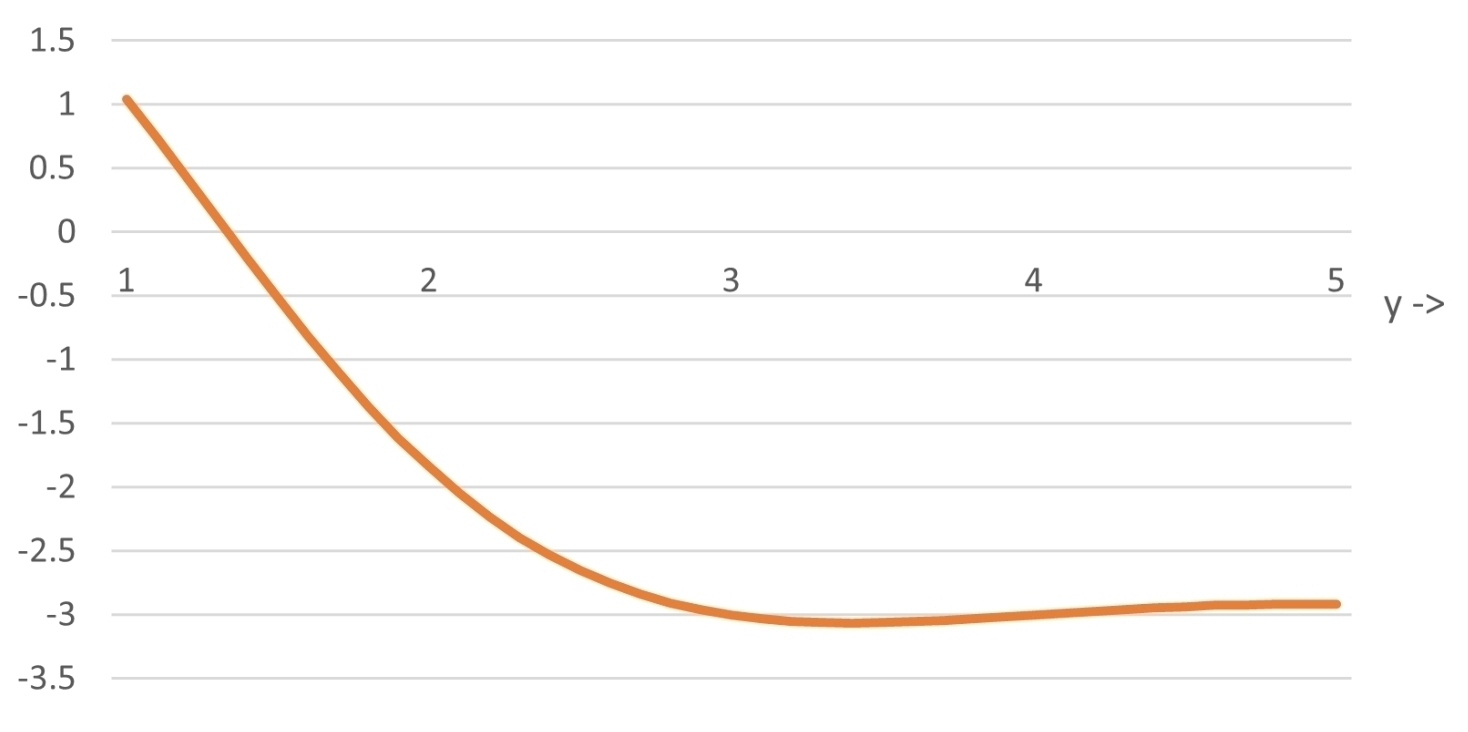
\includegraphics[width=0.7\linewidth]{ly2_continuous.jpg}
  \caption{Continuous variation of $L(y,2)$ with $y$}
\end{figure}

\begin{figure}[H]
  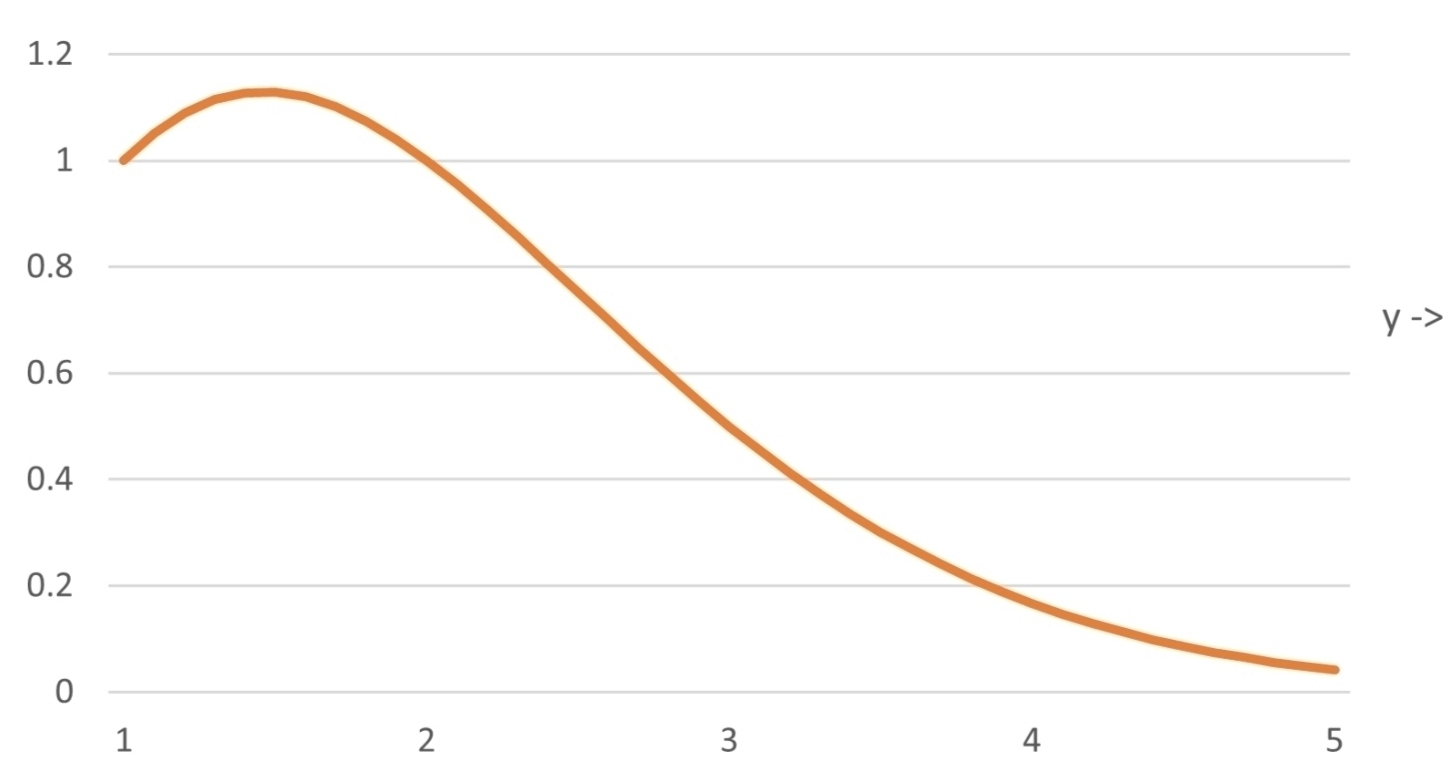
\includegraphics[width=0.7\linewidth]{residue_curve.jpg}
  \caption{Continuous variation of $\Res(\frac{1}{\log^{y} z},1)$ with y}
\end{figure}

On a continous scale, we see above how $L(y,2)$ and the residue at $z=1$ varies with $y$\\. 

$L(y,2)$ seems to have a local minima at 3.40776.. and a local maxima at 4.90184.. Beyond this the function seems to be monotonically decreasing with y.

$\Res(\frac{1}{\log^{y} z},1)$ seems to have a global maxima at y=1.46163.. where the residue acquires the maximum value 1.12917.. Beyond this, as y varies, the residue curve seems to monotonically decrease towards 0.


\section{Roots of $L(q,x)$ for real $q$}

As we did in an earlier section, we now compute the roots of $L(q,x)$ for real $q$ (under the assumption that $L(q,x)$ is real for real $q$, which as we saw in the previous section has good support).

\begin{table}[H]
    \begin{tabular}{r|r|r} % <-- Alignments: 1st column left, 2nd middle and 3rd right, with vertical lines in between
      $q$ & $\mu_{q}$ & $\frac{\mu_{q}}{\mu_{q-1}}$\\
      \hline
      0.51 & 1.000669 & \\
      0.55 & 1.012343 & \\
      0.6 & 1.039038 & \\
      0.7 & 1.115064 & \\
      0.8 & 1.211222 & \\
      0.9 & 1.323609 & \\
      1.0 & 1.451369 & \\
      1.1 & 1.594820 & \\
      1.2 & 1.754878 & \\
      1.3 & 1.932839 & \\
      1.4 & 2.130296 & \\
      1.5 & 2.349101 & \\
      2.0 & 3.846468 & 2.650234\\
      2.5 & 6.319568 & 2.690207\\
      3.5 & 17.118296 & 2.708776\\
      4.5 & 46.451592 & 2.713564\\
    \end{tabular}
    \caption{Roots of $L(q,x)$ for real $q$}
\end{table}
\vspace{-2em}
As seen in the table below, as $q \to 0.5$, $\mu_{q} \to 1$. Since $\frac{1}{log^{q} x}$ has a singularity at $1$, and $L(q,x)$ was defined for $x>1$, this implies no roots of $L(q,x)$ for $0<q<=0.5$.

Additionally, it can be seen that the roots for fractional exponents interpolate well between those for integer exponents, and the ratio of roots with $q_2 - q_1 = 1$ still converges towards $\e$, further providing confirmation that the behavior of $L(q,x)$ is not fundamentally different between integer and non-integer exponents.

\begin{figure}[H]
  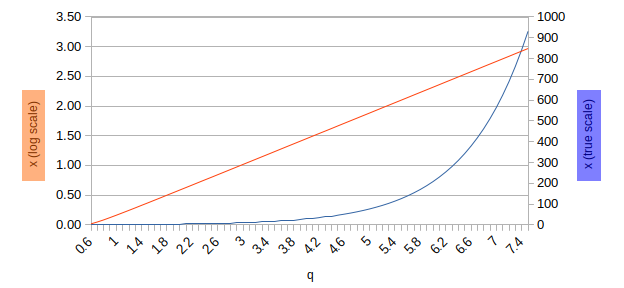
\includegraphics[width=0.5\linewidth]{logpowrealroots.png}
  \caption{Roots of $L(q,x)$ for real $q$}
\end{figure}

\section{$L(y,z)$ for complex $z$}

In our analysis so far, we used the constraint $x > 1$. Given that $\li(z)$ can also be defined for complex $z$, we now derive expressions for the full analytic continuation $L(y,z)$ defined everywhere except at $z=1$.

Starting from $L(y,z) = \int_0^z \frac{1}{\log^y t} dt$ and applying the variable change $t = \e^u$ and swapping the limits, we obtain:
\begin{align}
L(y,z) =& \int_{-\log(z)}^{\infty} \frac{\e^{-u}}{(-u)^y} \,du  \\ 
\notag \\
 =&\, (-1)^{-y}\,\int_{-\log(z)}^{\infty} \frac{\e^{-u}}{u^y} \,du \qquad \Re(y) \geq 0  
\end{align}

This integral already starts to show some resemblance with the generalised Exponential integral $\Ei$: 
\begin{equation}\label{rootscomp}
 \Ei(y,z) = z^{y-1}\,\int_z^{\infty} \frac{\e^{-u}}{u^y} du
\end{equation}

and to complete it, we multiply the integral by $(-1)^y = -\left(\log(z)\right)^{1-y}\,(-\log(z))^{y-1},\, \Re(z) \ge 0$, which gives: 
\begin{equation}\label{rootscomp1}
  L(y,z) = -\left(\log(z)\right)^{1-y}\,\Ei\left(y, -\log(z)\right)
\end{equation}

and this provides the analytic continuation towards $y \in \mathbb{C}, z \in \mathbb{C}, z \ne 1$. Note that when $z \in \mathbb{R}, z > 1$ a single term $\pi i$ needs be subtracted to accommodate for the branch cut when passing $z = 1$.

Focusing only on the real part and making $y$ an integer: $\RL(n,z) = \Re(L(n,z))$ we see that $\RL(n,z)$ has $n+1$ zeros, $n$ on the negative axis and one on the positive axis. The root for $\RL(1,z)=-2.46641..$ is already known \cite{oeis1}, while those for $n>=2$ appear new.

\begin{table}[H]
  \begin{center}
    \begin{tabular}{r|r} % <-- Alignments: 1st column left, 2nd middle and 3rd right, with vertical lines in between
      $n$ & root of RL(n,z)\\
      \hline
      1 & -2.46641\\
      \hline
      2 & -0.08544\\&-95.0475\\
      \hline
      3 & -0.00835\\&-2.15435\\&-1352.1909\\
    \end{tabular}
  \end{center}
  \caption{Negative axis zeros of $\RL(n,z)$}
\end{table}
\vspace{-2em}

We also observe that the function $M(n,z) = L(n,z) + L(n,1-z)$ has $n$ complex roots, that we conjecture to be all on the critical line $\Re(z)=0.5$.

\begin{table}[H]
  \begin{center}
    \begin{tabular}{r|r} % <-- Alignments: 1st column left, 2nd middle and 3rd right, with vertical lines in between
      $n$ & root of M(n,z)\\
      \hline
      1 & 0.5 + 0.51309i\\
      \hline
      2 & 0.5 + 0.28070i\\&0.5 + 2.33197i\\
      \hline
      3 & 0.5 + 0.19021i\\&0.5 + 0.86051i\\&0.5 + 7.48332i\\
    \end{tabular}
  \end{center}
  \caption{Roots of $M(n,z)$}
\end{table}
\vspace{-2em}

\section{Integrals of $L(y,z) = \IL^{(n)}(y,w)$}

With the 'closed form' expression derived in the previous section, we can now compute the $n$-th integral of $L(y,z) = \IL^{(n)}(y,w)$. We start from the Riemann-Liouville expression for multiple integrals:

\begin{equation}\label{rootscomp2}
\IL^{(n)}(y,w) = -\frac{1}{\Gamma(n)}\,\int_{0}^{w} \frac{\left(\log(z)\right)^{1-y}\,\Ei\left(y, -\log(z)\right)}{(w-z)^{1-n}}\, dz
\end{equation}

that can be transformed into the series when $n \in \mathbb{N}$:
\begin{equation}\label{rootscomp3}
\IL^{(n)}(y,w) = \frac{\left(\log(w)\right)^{1-y}}{\Gamma(n+1)}\,\sum_{k=1}^{n+1} (-1)^k\, \binom{n}{k-1}\,w^{n+1-k} \,\Ei\left(y, -k\log(w)\right)
\end{equation}

and simplified further into:
\begin{equation}\label{rootscomp4}
\IL^{(n)}(y,w) = \left(\log(w)\right)^{1-y}\,\sum_{k=1}^{n+1} \frac{(-1)^k\,w^{n+1-k}}{\Gamma(k)\,\Gamma(n+2-k)} \,\Ei\left(y, -k\log(w)\right)
\end{equation}
which is valid for $y,w \in \mathbb{C}, w \ne 1$.

This expression reveals a few more constants, for instance:

1) When we change $n$, whilst keeping $y=1, w \rightarrow 1$, we obtain the following sequence for an increasing number of integrals of $\li(z)$:
\begin{align}
\lim_{w^{-} \to 1} \IL^{(1)}(1,w) &= -\frac{1}{1}\log\left(\frac{2}{1}\right) \notag\\
\lim_{w^{-} \to 1} \IL^{(2)}(1,w) &= -\frac{1}{2}\,\log\left(\frac{4}{3}\right) \notag\\
\lim_{w^{-} \to 1} \IL^{(3)}(1,w) &= -\frac{1}{6}\,\log\left(\frac{32}{27}\right) \notag\\
\lim_{w^{-} \to 1} \IL^{(4)}(1,w) &= -\frac{1}{24}\,\log\left(\frac{4096}{3645}\right) \notag\\
\cdots \notag\\ 
\lim_{w^{-} \to 1} \IL^{(n)}(1,w) &= \sum_{k=1}^n \frac{(-1)^k\,\log(k+1)}{\Gamma(k+1)\,\Gamma(n+1-k)} \\ 
\notag
\end{align} 
The fractions inside the logs are OEIS: A122214 \cite{oeis2} and appear in infinite products for $\pi/2$, $e$ and $e^\gamma$.

2) Changing $n$ with $w \rightarrow 1$, yields a closed form for $y \in \mathbb{C}, y \notin \mathbb{N}$:

\begin{equation}\label{rootscomp5}
\lim_{w^{-} \to 1} \IL^{(n)}(y,w) = (-1)^{1-y}\,\Gamma(1-y)\,\sum_{k=1}^{n+1} \frac{(-1)^k\,k^{y-1}}{\Gamma(k)\,\Gamma(n+2-k)} 
\end{equation}
The case $n=0, y=1/2, w \rightarrow 1$ yields:
\begin{equation}\label{rootscomp6}
\lim_{w^{-} \to 1} L(1/2,w) = -i\sqrt{\pi}
\end{equation}
and for $n=0, y=-1/2, w \rightarrow 1$ we find:
\begin{equation}\label{rootscomp7}
\lim_{w^{-} \to 1} L(-1/2,w) = \frac{i\sqrt{\pi}}{2}
\end{equation}
For $n=1$, the function reduces to:
\begin{equation}\label{rootscomp8}
 \lim_{w^{-} \to 1} \IL^{(1)}(y,w) = (-1)^{1-y} \left(2^{y-1}-1\right)\Gamma(1-y)
 \end{equation} 
It is already known that $\int\limits_{0}^{1} \li(x)\, dx = -\ln(2)$ and this result is indeed obtained when $y \rightarrow 1$. Furthermore, when we take $y = m+\frac12$, $m = $ integer, this yields: 
\begin{equation}\label{rootscomp9}
\lim_{w^{-} \to 1} \IL^{(1)}(m,w) = \frac{2^{2m-1/2} - 2^m}{(2m - 1)!!} \sqrt{\pi}\, i 
\end{equation}
where $(f)!!$ is the double factorial.

\pagebreak
\section{Roots of the integrals of $L(y,z) = \IL^{(n)}(y,w)$}

The expression derived in the previous section enables us to compute where the real part of $\IL^{(n)}(y,w)$ becomes zero for various $y$ and $n$ in the domain $w > 1$. The table below lists the roots for some of these combinations:

\begin{table}[H]
  \begin{center}
    \begin{tabular}{r|r|r|r|r} % 
      root of:      &  &  &  & \\
      	\hline
		$\Re(\IL^{(1)}(1,w))$  &          &          &          &  2.611139 \\
		$\Re(\IL^{(1)}(2,w))$  &          &          & 1.093879 &  9.195551 \\
		$\Re(\IL^{(1)}(3,w))$  &          &          & 1.518154 & 27.944624 \\
		$\Re(\IL^{(1)}(4,w))$  &          &          & 2.260667 & 80.487321 \\
		\hline
		$\Re(\IL^{(2)}(1,w))$  &          &          &          &  3.793700 \\  
		$\Re(\IL^{(2)}(2,w))$  &          &          & 1.389081 & 14.537535 \\
		$\Re(\IL^{(2)}(3,w))$  &          & 1.041562 & 2.393445 & 45.540297 \\
		$\Re(\IL^{(2)}(4,w))$  &          & 1.227633 & 4.078447 &133.107773 \\
		\hline
		$\Re(\IL^{(3)}(1,w))$  &          &          &          &  4.980328 \\
		$\Re(\IL^{(3)}(2,w))$  &          &          & 1.712136 & 19.877496 \\
		$\Re(\IL^{(3)}(3,w))$  &          & 1.187160 & 3.254921 & 63.145216 \\
		$\Re(\IL^{(3)}(4,w))$  & 1.023554 & 1.615337 & 5.846396 &185.793844 \\ 
		\hline
		$\Re(\IL^{(4)}(1,w))$  &          &          &          &  6.168382 \\
		$\Re(\IL^{(4)}(2,w))$  &          &          & 2.043688 & 25.216529 \\
		$\Re(\IL^{(4)}(3,w))$  &          & 1.356665 & 4.113401 & 80.753065 \\
		$\Re(\IL^{(4)}(4,w))$  & 1.111856 & 2.000238 & 7.603218 &238.502648 \\ 
    \end{tabular}
  \end{center}
  \caption{Roots of $\Re(\IL^{(n)}(y,w))$}
\end{table}
\vspace{-2em}

The number of roots clearly varies dependent on the choice of $n, y$. The roots in the last column seem to converge to a growth factor $\e$ and the column before it by a factor $\sqrt{\e}$. We conjecture that the growth in the second column converges to $\sqrt{\sqrt{\e}}$, etc.


  
\section{Concluding Remarks and Future Work}

Since the zeta function $\zeta(s)$ shares the property with $\frac{1}{log x}$ of also having a simple pole at 1, we can repeat the entire analysis above for $\zeta^{y}(s)$. This will be explored in a different paper. Similarly, other functions of interest will be treated in subsequent papers. 

\begin{thebibliography}{99} 

\bibitem{edwr}
H.M. Edwards, \emph{Riemann's zeta function}, (1974), pg.85
\bibitem{rama}
S. Ramanujan, \emph{Collected Papers of Srinivasa Ramanujan}, Ed. G.H Hardy, P.V.S. Aiyar, B.M. Wilson. Providence, RI, Amer. Math. Soc., (2000), pg.351.
\bibitem{weis}
Weisstein, Eric. W \emph{Logarithmic Integral}, From Mathworld A Wolfram Web Resource which can be found at: https://mathworld.wolfram.com/LogarithmicIntegral.html)
\bibitem{oeis1}
OEIS A257821 \emph{Decimal expansion of the unique real number a>0 such that the real part of li(-a) is zero}, which can be found at: (https://oeis.org/A257821)
\bibitem{oeis2}
OEIS A122214 \emph{Numerators/denominators of fractions in infinite products for $\pi/2$, $e$ and $e^\gamma$ }, which can be found at: (https://oeis.org/A122214)
\end{thebibliography} 

\pagebreak

\appendix
\appendixpage
The below codes are in parigp language. As a cautionary practice while copy-pasting code, do check whether special characters like \textasciicircum \, (power symbol) have been copied too. Also it is a good practice to manually set parigp default parameters at the beginning of the code, as shown below.

\section{Example of setting default parameters for a parigp session}
Here we set defaults for power series representation, memory, and precision. There can be other kinds of default parameters as well.
\begin{verbatim}
default(seriesprecision,60);
default(parisizemax,100000000);
default(realprecision,100);
\end{verbatim}


\section{Contour integration on an open arc}
parigp has an inbuilt function intcirc for contour integration on a circular contour. 
We define a similar looking function intarc for integration on an open arc.

\begin{verbatim}
intarc(a,R,th1,th2,f,n) = intnum(t=th1,th2,I*R*exp(I*t)*f(a+R*exp(I*t),n))\
                          /((th2-th1)*I);
\end{verbatim}

Example computation
\begin{verbatim}
f(z,n) = 1/log(z)^n;
cpvsemi = Pi*I*intarc(1,1,0,Pi,f,3)
\end{verbatim}

\section{Getting the laurent coefficients for a function with a simple pole}
\begin{verbatim}
getlaurent(f,pole,maxind=3) = {
  lser = [];
  for(ind=-1,maxind,lser=concat(lser,polcoef(f(z+pole),ind)););
  return(lser);
}
\end{verbatim}

\section{Computing t-vectors}
t-vector computation is a combinatorial problem, and can be solved through multiple approaches. Conceptually simplest are brute force methods but they can be quite slow. Below we used a linear diophantine framework, which was found to scale much better.

\begin{verbatim}
ldsolve(ts,maxind,coeffs) = {
   local(allsols=List()); 
   if(maxind==1, 
      if(ts%coeffs[maxind]==0, listput(allsols,[ts/coeffs[maxind]]););    
      return(allsols);
   ); 
   tmax = floor(ts/coeffs[maxind]);
   for(t=0,tmax,
      rs=ts-t*coeffs[maxind];
      if(rs==0,
          sol=concat(vector(maxind-1,n,0),t);
          listput(allsols,sol);
          ,
          rsol = ldsolve(rs,maxind-1,coeffs); 
          for(m=1,#rsol,
                  sol=concat(rsol[m],t);
                  listput(allsols,sol);
          );
       );
   );
   return(allsols);
}

tvectors(k) = {
   coeffs=vector(k-2,n,n+1);
   ldsols = ldsolve(k-1,k-2,coeffs);
   local(tvecs = List());
   for(ind=1,#ldsols,
       sol=ldsols[ind];
       am=k-vecsum(sol);
       sol=concat(am,sol);
       listput(tvecs,sol);
   );
   return(tvecs);
}
\end{verbatim}

\section{Computing $\Res(f^{q}(z),c)$ with $q$ real, and $f(z)$ having a simple pole at $c$}

This generally works well when $q$ is either an integer or large real. For low real exponents, it may not converge.
  
\begin{verbatim}
fastresidue(baselaurent,q) = {
  bl=#baselaurent;
  am = baselaurent[1];
  a0 = baselaurent[2];
  arem = vecextract(baselaurent,vector(bl-2,n,n+2));
  avec = concat(am,arem);

  res=q*a0^(q-1)*am;

  for(k=3,bl,
    mult1 = binomial(q,k);
    mult2 = a0^(q-k);
    mult3 = 0;
    combs = tvectors(k);
    for(m=1,#combs,
          pr=combs[m];
          mterm=k!;
          for(j=1,k-1,mterm = mterm*(avec[j]^pr[j])/(pr[j]!););
          mult3=mult3+mterm;
    );
    res = res + mult1*mult2*mult3;
  );
return(res);
}
\end{verbatim}

\section{Computing $L(q,x)$ and $\Res(\frac{1}{\log^{q} z}, 1)$ for real $q$}
Here we use $q=15$ as an the large exponent anchor. A higher anchor can give more accurate results, but the computation is slower. For $q>=15$, L(q,x) is evaluated directly from the contour integral and residue estimates, while for $q<15$, we use recursion between $L(q,x)$ and $L(q+1,x)$.\\
Similarly by default we use the laurent terms from $a_{-1}$ to $a_{30}$ of the base function $\frac{1}{\log x}$. More laurent terms should give more accuracy at the cost of computation speed.

\begin{verbatim}
rlog(z) = 1/log(z);

L(q,x,lterms=30) = {
    if(q<15,
       return(q*L(q+1,x,lterms) + x*rlog(x)^q);
       ,
       contint=intnum(t=0,Pi,I*exp(I*t)*rlog(1+exp(I*t))^q,1);
       remint=intnum(v=2,x,rlog(v)^q,1);
       res = fastresidue(getlaurent(rlog,1,lterms),q);
       return(-contint + res*Pi*I + remint);
      );
}

lpres(q,lterms=30) = (intnum(t=0,Pi,I*exp(I*t)*rlog(1+exp(I*t))^q,1) + \
                                    L(q,2,lterms))/Pi/I;
\end{verbatim}

\section{Calculating roots of $L(n,x)$ for integer $n$}
With some easy modifications, the same can be done for real q as well, which we leave as an exercise for the reader.

\begin{verbatim}
{
zprev=1;
for(y=1,40,
   zero=solve(x=1.1,10^50,L(y,x));
   print(y,",",zero,",",zero/zprev);
   zprev=zero;
   );
}   
\end{verbatim}

\section{Finding extrema of $L(y,2)$ and $\Res(\frac{1}{\log^{y} z}, 1)$}
We do not have closed form expressions for derivatives of L(y,2) and $\Res(\frac{1}{\log^{y} z}, 1)$, hence to calculate extrema, we can either approximate the derivative using Newton's quotient with h small enough to meet precision requirements, or use gp's inbuilt derivative operator ', which does the same thing.

\begin{verbatim}
f(s,y) = 1/log(s)^y;
g(x,y) = intnum(s=x,2,f(s,y));
L(y,x) = -real(Pi*I*intarc(1,1,0,Pi,f,y)) - g(x,y);
lpres(y) = real(intarc(1,1,0,Pi,f,y));
solve(y=1,4,L'(y,2))
solve(y=4,8,L'(y,2))
solve(y=1,4,lpres'(y))
\end{verbatim}


\end{document}
